% !TEX root = main.tex

\section{调度}
\subsection{单处理器调度}
三级调度层次
\begin{itemize}
    \item 长程调度(Long-term scheduling)/任务调度
    \begin{itemize}
    \item 决定哪些新建进程可进入系统\textbf{准备执行}(ready)
    \item 控制多道程序系统的并发程度
    \item 进程越多则各进程对CPU的使用百分比越小
    \end{itemize}
    \item 中程调度(Medium-term scheduling)
    \begin{itemize}
    \item 决定交换哪些主存-辅存(内存-外存)进程
    \item 基于多道程序设计的管理需要
    \end{itemize}
    \item 短程调度(Short-term scheduling)/CPU调度
    \begin{itemize}
    \item 决定下一个使用CPU的进程(dispatcher,分派程序)
    \end{itemize}
\end{itemize}

\begin{figure}[H]
    \centering
    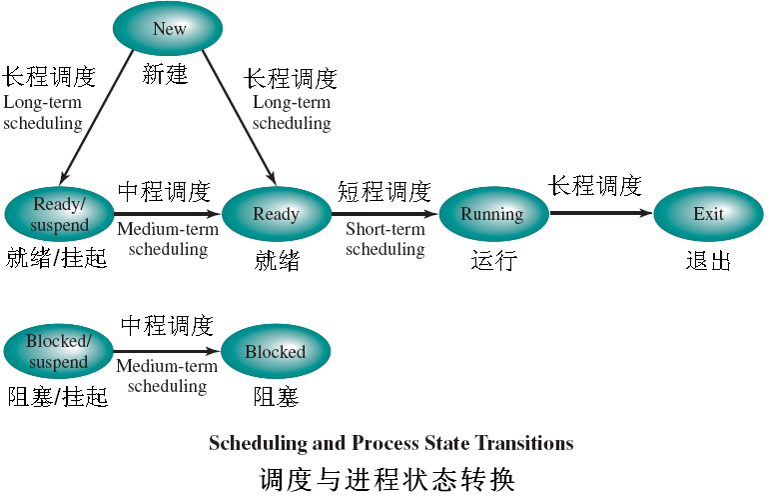
\includegraphics[width=0.6\linewidth]{fig/process_scheduling.png}
\end{figure}

进程调度方式
\begin{itemize}
    \item 剥夺式:立即分配
    \item 非剥夺式:当前进程执行完再分配给新进程
\end{itemize}

评价指标:
\begin{itemize}
\item 周转时间/驻留时间$T_r$:作业\textbf{提交到完成}所经历的时间,等待时间+服务时间
\item 归一化周转时间:周转时间与服务时间的比值,表示一个进程的相对延迟情况
\item 吞吐量:单位时间内\textbf{完成的进程数量}
\end{itemize}

进程短程调度算法
\begin{itemize}
\item 先来先服务(First Come First Served,FCFS):公平,更有利于CPU密集型和长作业,不利于短作业
\item 时间片轮转(time slicing Round Robin,RR):最公平,兼顾长短作业,也是剥夺式调度(时间片用完时);平均等待时间较长,上下文切换浪费时间,对IO密集型进程最不利
\item 虚拟时间片轮转(VRR):进程因IO而阻塞会进入到专门的IO队列中,解除了IO阻塞的进程会被转移到一个FCFS的辅助队列中。进行调度决策时,辅助队列中的进程优先于就绪队列中的进程。提升了公平性。
\begin{figure}[H]
    \centering
    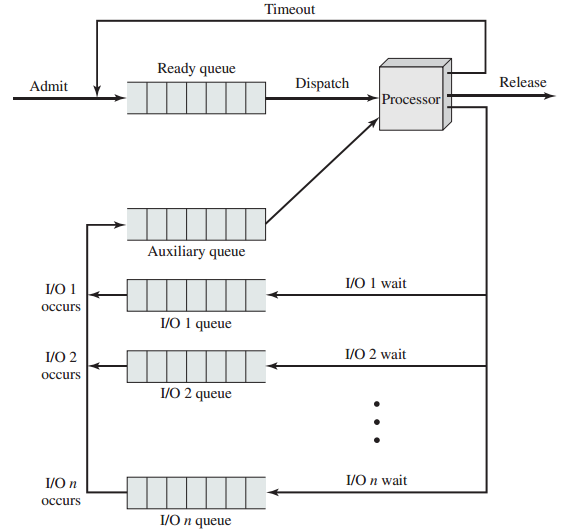
\includegraphics[width=0.6\linewidth]{fig/VRR.png}
\end{figure}
\item 最短进程优先(Shortest Process Next,SPN):非抢占式策略,但需要用EWMA预测,吞吐量最大,长作业会饥饿
\[S_{n+1}=aT_n+(1-a)S_n\]
\item 最短剩余优先(Shortest Remaining Time,SRT):SPN结合\textbf{抢占策略};但必须记录过去的服务时间,增加开销
\item 最高响应比优先(Highest Response Ratio Next,HRRN):兼顾长短作业,计算响应比开销大,\textbf{非剥夺型};注意$T_{wait}$是截至当前等待处理器的时间,因此长进程由于得不到服务,$R_P$会一直增加,最终在竞争中胜过短进程。
\[R_P=\frac{T_{wait}+T_{serve}}{T_{serve}}\]
\item 最高优先级优先(Highest Priority First,HPF)
\item 多级队列反馈(Multilevel Feedback,MF/FB):结合FCFS、RR和HPF,设置多条优先级不同的队列,前面的队列用FCFS,最后一条队列用RR;每次时间片到都会降级到下一个优先级中,短进程很快执行完毕,而长进程则会多次降级;$q=1$类似于时间片为1的轮转法,$q=2^i$则是对于第$i$个队列,可以执行$q=2^i$个周期才被抢占
\begin{figure}[H]
    \centering
    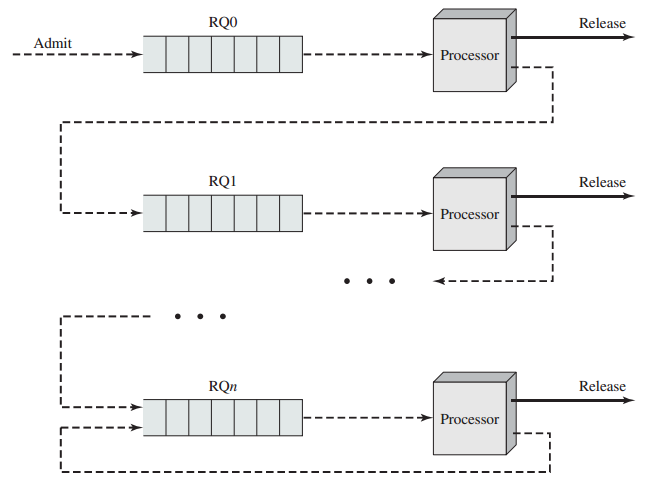
\includegraphics[width=0.6\linewidth]{fig/feedback.png}
\end{figure}
\end{itemize}

\begin{example}
    考虑下面的进程
    \begin{center}
        \begin{tabular}{|c|c|c|}\hline
            进程 & 到达时间 & 服务时间\\\hline
            A & 0 & 3\\\hline
            B & 2 & 6\\\hline
            C & 4 & 4\\\hline
            D & 6 & 5\\\hline
            E & 8 & 2\\\hline
        \end{tabular}
    \end{center}
\end{example}
\begin{analysis}
    有下面的时序图
    \begin{figure}[H]
        \centering
        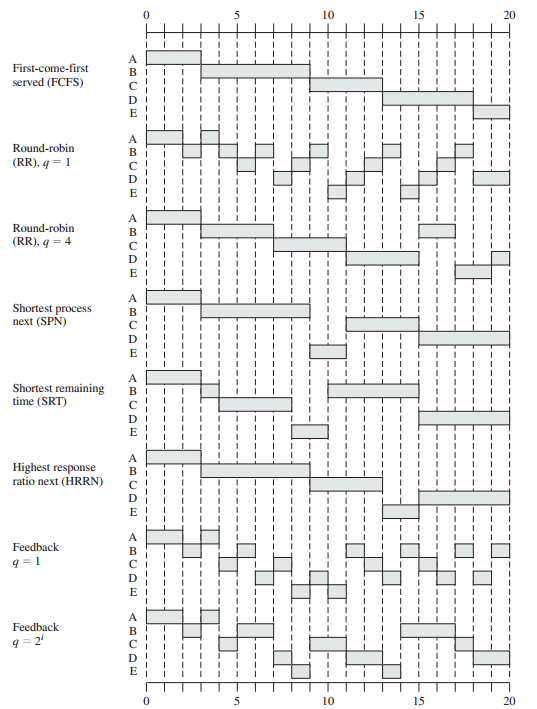
\includegraphics[width=0.8\linewidth]{fig/short-term-scheduling-all.png}
    \end{figure}
    \begin{figure}[H]
        \centering
        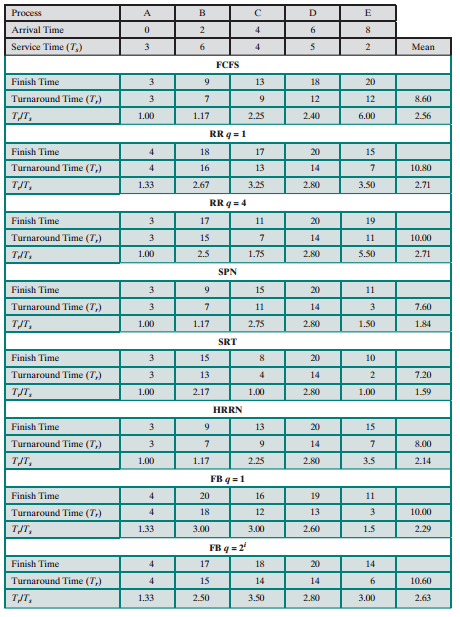
\includegraphics[width=0.8\linewidth]{fig/short-term-scheduling-all-2.png}
    \end{figure}
\end{analysis}

\subsection{多处理器调度}
多处理器线程调度方案
\begin{itemize}
    \item 负载共享(load sharing)
    \item 组调度(gang scheduling)
    \item 专用处理器分配
    \item 动态调度
\end{itemize}

\subsection{调度算法总结}
\begin{itemize}
    \item 动态分区放置算法:First-fit、Best-fit、Next-fit
    \item 页的替换策略:Opt、LRU、FIFO、Clock
    \item 单处理器进程调度:FCFS、SPN、SRT、HRRN、RR、HPF、MF/FB
    \item 磁盘调度算法:FCFS、SSTF、SCAN、C-SCAN
\end{itemize}

% 填空10*2
% 简答题6*5
% 应用题5